\documentclass[aspectratio=169,10pt]{beamer}
\usepackage[T1]{fontenc}
\usepackage[utf8]{inputenc}
\usepackage{amsmath,amssymb,booktabs,graphicx,xcolor,array}
\usepackage{tikz}
\usetikzlibrary{positioning,arrows.meta,shapes.geometric,fit,calc}
\graphicspath{{figures/}}

\definecolor{navy}{HTML}{1F4E79}
\definecolor{teal}{HTML}{1B7F79}
\definecolor{warm}{HTML}{B5651D}
\definecolor{soft}{HTML}{EAF1F8}
\definecolor{muted}{HTML}{5A6572}

\usetheme{default}
\usefonttheme{professionalfonts}
\setbeamertemplate{navigation symbols}{}
\setbeamercolor{structure}{fg=navy}
\setbeamercolor{frametitle}{fg=navy,bg=white}
\setbeamercolor{title}{fg=navy}
\setbeamercolor{itemize item}{fg=teal}
\setbeamercolor{block title}{bg=navy,fg=white}
\setbeamercolor{block body}{bg=soft,fg=black}
\setbeamerfont{frametitle}{series=\bfseries,size=\large}
\setbeamerfont{block title}{size=\small,series=\bfseries}
\setbeamertemplate{frametitle}{%
  \vskip2.5mm\hskip-0.5mm\usebeamercolor[fg]{frametitle}\usebeamerfont{frametitle}\insertframetitle\par
  \vskip0.8mm{\color{navy}\hrule height 0.8pt}\vskip1mm}
\setbeamertemplate{footline}{%
  \hfill{\color{muted}\scriptsize ToF-SIMS PCA \quad\insertframenumber/\inserttotalframenumber}\hspace{4mm}\vskip3mm}
\setlength{\leftmargini}{1.1em}

\newcommand{\hl}[1]{{\color{warm}\bfseries #1}}
\newcommand{\src}[1]{{\color{muted}\scriptsize #1}}

\tikzset{
  box/.style={draw=navy,fill=soft,rounded corners=2pt,align=center,font=\scriptsize,minimum height=9mm,inner sep=2.5pt},
  boxw/.style={box,fill=white},
  hi/.style={box,fill=navy,text=white,draw=navy},
  hw/.style={box,fill=warm!15,draw=warm},
  arr/.style={-{Stealth[length=2mm]},navy,thick}
}

\title{PCA of ToF-SIMS spectra}
\subtitle{Preprocessing transformations, All-peak PCA and Selected-peak PCA}
\author{Jose Tupayachi}
% \institute{Oak Ridge National Laboratory}
\date{\today}

\begin{document}

\begin{frame}[plain]
  \vspace{8mm}
  \begin{center}
    {\color{navy}\Large\bfseries PCA of ToF-SIMS spectra}\\[2mm]
    {\color{teal}\large Preprocessing transformations, All-peak PCA and Selected-peak PCA}\\[7mm]
    % {\small Jose Tupayachi \quad$\cdot$\quad Oak Ridge National Laboratory}\\[1mm]
    {\color{muted}\small \today}
    \vfill
    % {\color{muted}\scriptsize Method: Yang et al., Biointerphases 14, 051004 (2019) \quad$\cdot$\quad Criteria: Fu et al., Atmos.\ Environ.\ 191, 36 (2018)\\
    % Figures: real data processed with \texttt{tof\_sims\_driver} (positive polarity, 24 subsamples)}
  \end{center}
\end{frame}

\begin{frame}{Outline}
  \begin{enumerate}
    \setlength\itemsep{3mm}
    \item \hl{What PCA is}: Base definition
    \item \hl{The transformations} applied to the spectra before PCA: Bins, total-ion normalisation, square root, centring
    \item \hl{Two rounds of PCA} (Yang et al.): All-peak PCA, then Selected-peak PCA
    \item \hl{Our implementation} what differs from Yang
  \end{enumerate}
\end{frame}

% =============================================================== PART 1
\begin{frame}{The problem: too many variables per sample}
  \begin{columns}[T]
    \begin{column}{0.56\textwidth}
      \begin{itemize}\setlength\itemsep{2mm}
        \item A ToF-SIMS spectrum has hundreds of peaks. Each peak is one \hl{variable}.
        \item A set example: \hl{24 subsamples} $\times$ \hl{901 bins} (1~u bins up to m/z 900).
        \item Question: which samples are chemically similar, and which peaks make them different?
        \item Looking at 24 spectra by eye does not answer this. A table of $24\times 901$ numbers does not either.
        \item PCA is a standard way to summarise such data and is one of the most used methods for ToF-SIMS interpretation \src{(Sek et al.\ 2021)}.
      \end{itemize}
    \end{column}
    \begin{column}{0.4\textwidth}
      \begin{block}{Data matrix $X$}
        \[
        X=\begin{pmatrix}
        x_{11}&\cdots&x_{1p}\\
        \vdots&\ddots&\vdots\\
        x_{n1}&\cdots&x_{np}
        \end{pmatrix}
        \]
        rows $i$: subsamples ($n=24$)\\
        columns $j$: peaks or bins ($p=901$)\\
        entry $x_{ij}$: ion counts of bin $j$ in subsample $i$
      \end{block}
    \end{column}
  \end{columns}
\end{frame}

\begin{frame}{PCA}
  \begin{columns}[T]
    \begin{column}{0.52\textwidth}
      \begin{block}{Definition}
        PCA finds new axes, the \hl{principal components} (PCs), that are linear combinations of the original variables.
      \end{block}
      \begin{itemize}\setlength\itemsep{1.5mm}
        \item \hl{PC1} is the direction with the largest variance in the data.
        \item \hl{PC2} is the largest remaining direction, at a right angle to PC1. And so on.
        \item Each sample is projected on the first PCs. The result is a map where similar samples lie close together.
        \item It is \hl{unsupervised}: Group labels are not used to compute the axes.
      \end{itemize}
    \end{column}
    \begin{column}{0.44\textwidth}
      \begin{center}
      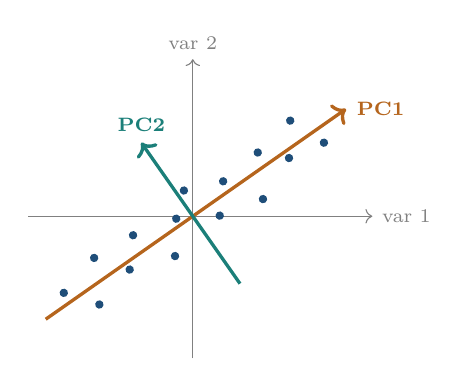
\begin{tikzpicture}[scale=0.95]
        \draw[->,gray] (-2.2,0) -- (2.4,0) node[right,font=\scriptsize] {var 1};
        \draw[->,gray] (0,-1.9) -- (0,2.1) node[above,font=\scriptsize] {var 2};
        \begin{scope}[rotate=35]
          \foreach \u/\v in {-2/0.15,-1.7/-0.25,-1.4/0.3,-1.1/-0.1,-0.8/0.25,-0.5/-0.3,-0.2/0.1,0.1/0.35,0.3/-0.2,0.6/0.15,0.9/-0.35,1.2/0.2,1.5/-0.1,1.8/0.3,2.0/-0.2}
            \fill[navy] (\u,\v) circle (1.6pt);
          \draw[->,warm,very thick] (-2.4,0) -- (2.5,0) node[right,font=\scriptsize\bfseries,warm] {PC1};
          \draw[->,teal,very thick] (0,-1.1) -- (0,1.2) node[above,font=\scriptsize\bfseries,teal] {PC2};
        \end{scope}
      \end{tikzpicture}\\[-1mm]
      {\scriptsize schematic: PC1 follows the long axis of the cloud}
      \end{center}
    \end{column}
  \end{columns}
\end{frame}

\begin{frame}{PCA}
  \small
  \begin{enumerate}\setlength\itemsep{2.2mm}
    \item \hl{Centre} each column:\quad $Z = X - \mathbf 1\,\bar{x}^{\!\top}$, \quad $\bar{x}_j=\tfrac1n\sum_i x_{ij}$
    \item \hl{Covariance} of the variables:\quad $C = Z^{\top}Z/(n-1)$
    \item \hl{Directions}: eigenvectors $C\,v_k=\lambda_k v_k$, orthonormal, with $\lambda_1\ge\lambda_2\ge\dots$\\
          Computed in practice by the singular value decomposition $Z = U S V^{\top}$, with $\lambda_k = s_k^2/(n-1)$
    \item \hl{Scores}: coordinates of the samples, $T = Z V = U S$\hfill one row per sample
    \item \hl{Explained variance}: $\mathrm{EV}_k=\lambda_k\big/\sum_l\lambda_l$
  \end{enumerate}
  \vspace{2mm}
  \begin{block}{Consequences}
    The loadings are the columns of $V$ (one weight per peak and PC). At most $\min(n-1,\,p)$ components exist.
    Because PCA maximises variance, \hl{variables with large variance dominate}, so the scaling of the data matters.
  \end{block}
\end{frame}

\begin{frame}{How to read a PCA result}
  \begin{columns}[T]
    \begin{column}{0.32\textwidth}
      \begin{block}{Scores}
        One point per \hl{subsample}, at its position on two PCs.\\[1mm]
        Points close together have similar spectra. Labels only colour the points.
      \end{block}
    \end{column}
    \begin{column}{0.32\textwidth}
      \begin{block}{Loadings}
        One weight per \hl{peak} and PC.\\[1mm]
        A large $|{\rm weight}|$ means the peak drives that axis. The sign gives the direction.
      \end{block}
    \end{column}
    \begin{column}{0.32\textwidth}
      \begin{block}{Explained variance}
        Share of the total variance carried by each PC (scree plot).\\[1mm]
        Tells how many PCs are worth looking at.
      \end{block}
    \end{column}
  \end{columns}
  \vspace{4mm}
  \begin{itemize}\setlength\itemsep{2mm}
    \item The axes are \hl{not} m/z. The m/z of a peak only appears in the loadings, where it says which peaks build each axis.
    \item Scores answer ``which samples differ'', loadings answer ``which peaks make them differ''.
  \end{itemize}
\end{frame}

\begin{frame}{Why spectra need preprocessing before PCA}
  PCA follows variance, so anything that inflates variance for the wrong reason distorts the result.
  \vspace{2mm}
  \begin{columns}[T]
    \begin{column}{0.32\textwidth}
      \begin{block}{Different total signal}
        Total ions per subsample range from \hl{18.8\,M to 86.4\,M} (4.6$\times$) in our set. PC1 could just reflect signal size.
      \end{block}
    \end{column}
    \begin{column}{0.32\textwidth}
      \begin{block}{Range}
        A few intense low-mass peaks carry most of the counts and would dominate the variance.
      \end{block}
    \end{column}
    \begin{column}{0.32\textwidth}
      \begin{block}{Counting noise}
        Ion counts are Poisson-like: the larger the count, the larger its random spread.
      \end{block}
    \end{column}
  \end{columns}
  \vspace{4mm}
  % \centering\large Remedy: \hl{total-ion normalisation}, \hl{square root} and \hl{mean centring}
\end{frame}

% =============================================================== PART 2
\begin{frame}{The transformation pipeline (as implemented)}
  \centering
  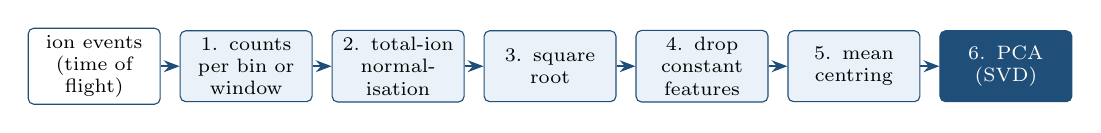
\begin{tikzpicture}[node distance=2.4mm]
    \node[boxw,text width=15mm] (a) {ion events (time of flight)};
    \node[box,text width=15mm,right=of a] (b) {1. counts per bin or window};
    \node[box,text width=15mm,right=of b] (c) {2. total-ion normalisation};
    \node[box,text width=15mm,right=of c] (d) {3. square root};
    \node[box,text width=15mm,right=of d] (e) {4. drop constant features};
    \node[box,text width=15mm,right=of e] (f) {5. mean centring};
    \node[hi,text width=15mm,right=of f] (g) {6. PCA (SVD)};
    \foreach \x/\y in {a/b,b/c,c/d,d/e,e/f,f/g} \draw[arr] (\x) -- (\y);
  \end{tikzpicture}
  \vspace{5mm}
  \begin{itemize}\setlength\itemsep{2mm}
    \item Order is fixed: \hl{normalise $\rightarrow$ square root $\rightarrow$ centre} (Yang et al.\ 2019).
    \item Steps 2 and 3 can be switched off in the app (\texttt{normalize = none}, \texttt{sqrt} off). Centring and the SVD always run.
    \item Peak-quality metrics (slide~\ref{sl:crit}) are computed on the \emph{raw} counts, before step 2.
    \item The same pipeline is used for the All-peak and the Selected-peak PCA. Only the features of step 1 differ.
  \end{itemize}
\end{frame}

\begin{frame}{Step 1: from ion events to a feature matrix}
  Each ion has a time of flight $t$; the calibrated mass is $m=\big((t-k_0)/s_f\big)^2$.
  \vspace{2mm}
  \begin{columns}[T]
    \begin{column}{0.5\textwidth}
      \begin{block}{All-peak PCA}
        Every bin of width $w$ is a feature:
        \[ x_{ij}=\#\{\text{ions of }i:\ j\,w\le m<(j+1)\,w\} \]
        $w=1$~u up to m/z 900 gives $p=901$ bins. No peak identification, no selection.
      \end{block}
    \end{column}
    \begin{column}{0.5\textwidth}
      \begin{block}{Selected-peak PCA}
        Only chosen peak windows are features:
        \[ x_{ip}=\#\{\text{ions of }i:\ lo_p\le m<hi_p\} \]
        one integrated count per peak, read directly from the time-of-flight channels.
      \end{block}
    \end{column}
  \end{columns}
  \vspace{3mm}
  Result: a matrix of raw counts $X$ with one row per subsample, kept for export before any transformation.
\end{frame}

\begin{frame}{Step 2: total-ion normalisation}
  \begin{block}{Formula}
    \[ \tilde{x}_{ij}=\frac{x_{ij}}{\sum_{k}x_{ik}} \qquad\Rightarrow\qquad \sum_j \tilde{x}_{ij}=1\ \text{ for every subsample } i \]
  \end{block}
  \begin{itemize}\setlength\itemsep{2mm}
    \item Each spectrum is divided by its own total, so rows describe \hl{composition}, not signal size.
    \item In the All-peak PCA the sum runs over all bins. In the Selected-peak PCA it runs over the \hl{selected peaks only}, as in Yang et al.\ (``normalised to the selected total ion intensity'').
    \item Our subsamples differ by up to 4.6$\times$ in total ions, which this step removes.
    \item App setting: \texttt{normalize = total-ion} (default) or \texttt{none}.
  \end{itemize}
\end{frame}

\begin{frame}{Step 3: square-root transform}
  \begin{block}{Formula}
    \[ y_{ij}=\sqrt{\tilde{x}_{ij}} \]
  \end{block}
  \begin{columns}[T]
    \begin{column}{0.34\textwidth}
      \begin{itemize}\setlength\itemsep{2mm}
        \item Compresses the \hl{dynamic range}: big peaks shrink most, small peaks gain relative weight.
        \item \hl{Variance stabilisation}: for Poisson counts the variance grows with the mean, while the variance of $\sqrt{\cdot}$ is roughly constant.
        \item App setting: \texttt{sqrt} on (default) or off.
      \end{itemize}
    \end{column}
    \begin{column}{0.64\textwidth}
      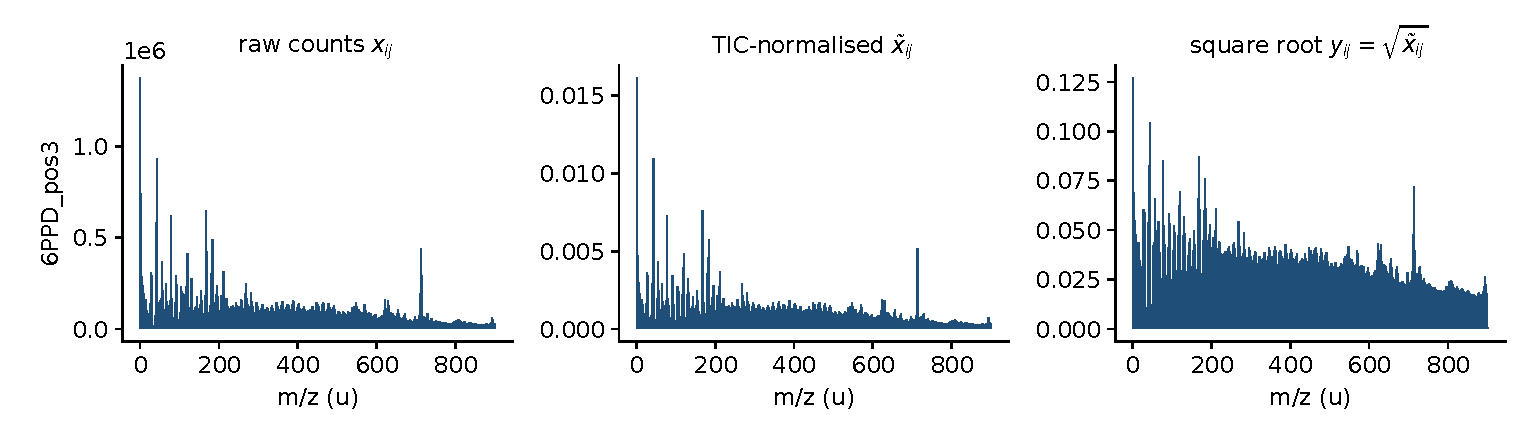
\includegraphics[width=\textwidth]{spectrum_steps.pdf}\\[-1mm]
      {\scriptsize One real spectrum (6PPD\_pos1, 1~u bins) at three stages. The shape is preserved, the dominance of the largest bins is reduced.}
    \end{column}
  \end{columns}
\end{frame}

\begin{frame}{Does the square root help on our data?}
  \centering
  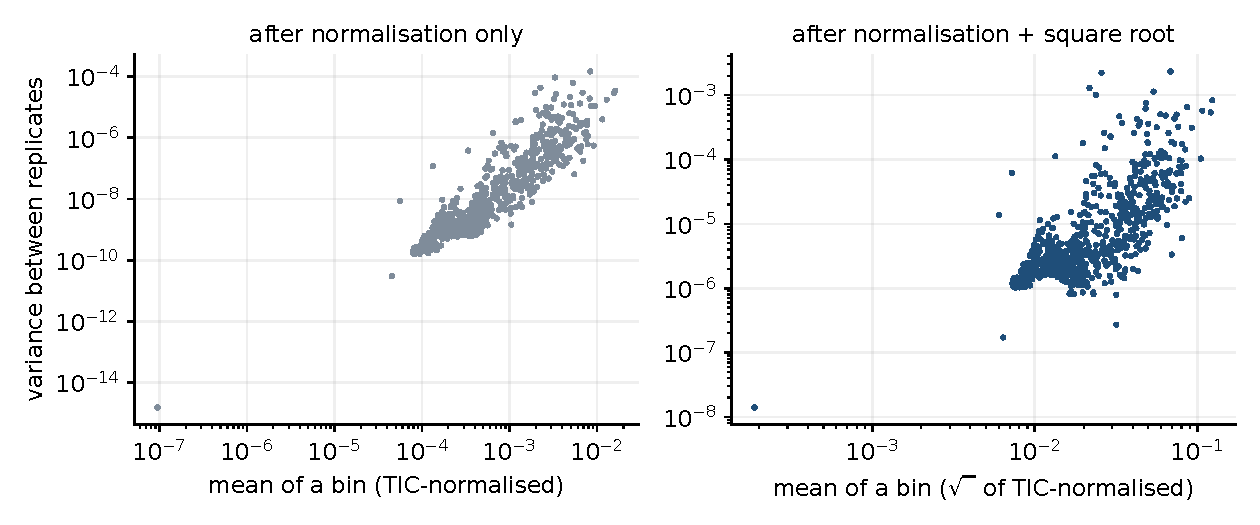
\includegraphics[width=0.7\textwidth]{variance_sqrt.pdf}
  \vspace{1mm}
  \begin{itemize}\setlength\itemsep{1.5mm}
    \item Each dot is one of the 901 bins: mean and variance over replicates, averaged over the five sample groups.
    \item The spread of the variance (1st to 99th percentile) is \hl{5.1 decades} after normalisation alone and \hl{2.8 decades} after the square root.
    \item The variance is compressed but not made constant: replicates also differ for reasons beyond counting noise.
  \end{itemize}
\end{frame}

\begin{frame}{Steps 4 and 5: drop constant features, centre the columns}
  \begin{columns}[T]
    \begin{column}{0.5\textwidth}
      \begin{block}{Drop constant features}
        \[ \text{keep } j \iff s_j=\mathrm{sd}_i(y_{ij})>0 \]
        Bins or peaks with no variation carry no information and are removed. All 901 bins were kept in our run.
      \end{block}
    \end{column}
    \begin{column}{0.5\textwidth}
      \begin{block}{Mean centring}
        \[ z_{ij}=y_{ij}-\bar{y}_j,\qquad \bar{y}_j=\tfrac1n\sum_i y_{ij} \]
        Puts the origin at the average spectrum. PCs then describe \hl{differences between samples}.
      \end{block}
    \end{column}
  \end{columns}
  \vspace{3mm}
  \begin{itemize}\setlength\itemsep{2mm}
    \item \hl{No unit-variance scaling} (z-score). Yang's recipe only centres. Dividing by $s_j$ would give every peak equal weight and inflate weak, noisy peaks.
    \item The PCA itself is the SVD of $Z$ (slide on PCA in five lines). Backend: GPU (cuML) if available, else scikit-learn, else numpy.
  \end{itemize}
\end{frame}

\begin{frame}{Worked example: 3 subsamples $\times$ 4 peaks}
  \scriptsize
  \begin{columns}[T]
    \begin{column}{0.5\textwidth}
      \textbf{Raw counts $x_{ij}$}\\[1mm]
      \begin{tabular}{@{}lrrrr|r@{}}
        \toprule & P1 & P2 & P3 & P4 & total\\\midrule
        S1 & 400 & 100 & 400 & 100 & 1000\\
        S2 & 900 & 200 & 600 & 300 & 2000\\
        S3 & 100 & 400 & 300 & 200 & 1000\\\bottomrule
      \end{tabular}\\[3mm]
      \textbf{Square root $y_{ij}$}\\[1mm]
      \begin{tabular}{@{}lrrrr@{}}
        \toprule & P1 & P2 & P3 & P4\\\midrule
        S1 & 0.632 & 0.316 & 0.632 & 0.316\\
        S2 & 0.671 & 0.316 & 0.548 & 0.387\\
        S3 & 0.316 & 0.632 & 0.548 & 0.447\\\bottomrule
      \end{tabular}
    \end{column}
    \begin{column}{0.5\textwidth}
      \textbf{Normalised $\tilde{x}_{ij}$}\\[1mm]
      \begin{tabular}{@{}lrrrr@{}}
        \toprule & P1 & P2 & P3 & P4\\\midrule
        S1 & 0.40 & 0.10 & 0.40 & 0.10\\
        S2 & 0.45 & 0.10 & 0.30 & 0.15\\
        S3 & 0.10 & 0.40 & 0.30 & 0.20\\\bottomrule
      \end{tabular}\\[3mm]
      \textbf{Centred $z_{ij}$}\\[1mm]
      \begin{tabular}{@{}lrrrr@{}}
        \toprule & P1 & P2 & P3 & P4\\\midrule
        S1 & 0.093 & $-$0.105 & 0.056 & $-$0.067\\
        S2 & 0.131 & $-$0.105 & $-$0.028 & 0.004\\
        S3 & $-$0.224 & 0.211 & $-$0.028 & 0.064\\\bottomrule
      \end{tabular}
    \end{column}
  \end{columns}
  \vspace{3mm}
  \normalsize
  \begin{itemize}\setlength\itemsep{1mm}
    \item S2 has twice the counts of S1, but after normalisation the two are close. S3 is different.
    \item PC1 explains \hl{95.6\%} of the variance and separates S3 from S1 and S2 (scores 0.155, 0.160, $-$0.315). With $n=3$ at most two PCs exist.
  \end{itemize}
\end{frame}

\begin{frame}{Summary of the transformations}
  \small
  \renewcommand{\arraystretch}{1.25}
  \begin{tabular}{@{}>{\raggedright\arraybackslash}p{2.8cm}>{\raggedright\arraybackslash}p{3.7cm}>{\raggedright\arraybackslash}p{3.9cm}>{\raggedright\arraybackslash}p{2.1cm}@{}}
    \toprule
    \textbf{Step} & \textbf{Formula} & \textbf{Purpose} & \textbf{App setting}\\\midrule
    Features & counts per bin or window & turn a spectrum into a row & bin width, peaks\\
    Total-ion normalisation & $\tilde{x}_{ij}=x_{ij}/\sum_k x_{ik}$ & removes total-signal differences & \texttt{normalize}\\
    Square root & $y_{ij}=\sqrt{\tilde{x}_{ij}}$ & tame dynamic range and counting noise & \texttt{sqrt}\\
    Drop constant & keep $j$ if $\mathrm{sd}(y_{\cdot j})>0$ & remove empty features & automatic\\
    Mean centring & $z_{ij}=y_{ij}-\bar{y}_j$ & origin at the mean spectrum & always\\
    PCA (SVD) & $Z=USV^{\top}$ & axes of maximal variance & components\\\bottomrule
  \end{tabular}
  \vspace{4mm}

  \normalsize
  \hl{Not applied:} logarithm, unit-variance scaling (z-score) and Pareto scaling. Only the steps above exist in the code.
\end{frame}

% =============================================================== PART 3
\begin{frame}{Two rounds of PCA: the idea of Yang et al.\ (2019)}
  \begin{columns}[T]
    \begin{column}{0.4\textwidth}
      \begin{itemize}\setlength\itemsep{2mm}
        \item Title: \emph{Peak selection matters in principal component analysis}.
        \item Question: how much does the choice of peaks change a spectral PCA?
        \item Samples: two \emph{Geobacter} species, alone and in coculture, plus two culture media (liquid ToF-SIMS).
        \item Same preprocessing in both rounds: normalise $\rightarrow$ square root $\rightarrow$ mean-centre.
        \item Round 1 uses \hl{all peak}, round 2 uses \hl{selected peak}.
      \end{itemize}
    \end{column}
    \begin{column}{0.58\textwidth}
      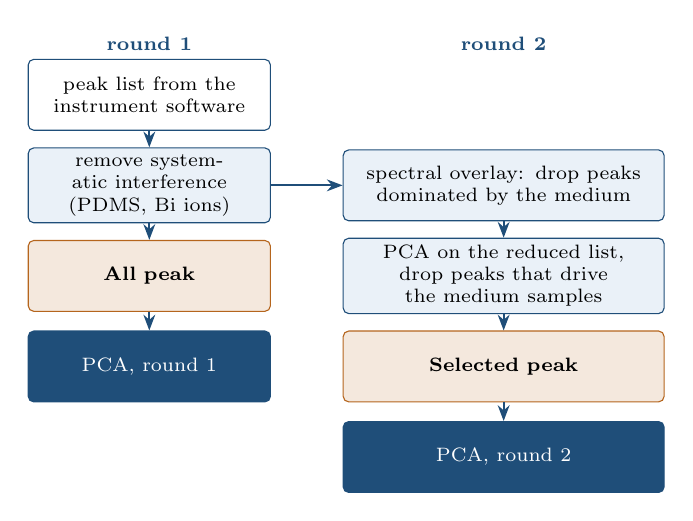
\begin{tikzpicture}[every node/.style={font=\scriptsize}]
        \node[boxw,text width=2.9cm] (l1) at (1.5,0) {peak list from the instrument software};
        \node[box,text width=2.9cm] (l2) at (1.5,-1.15) {remove systematic interference (PDMS, Bi ions)};
        \node[hw,text width=2.9cm] (l3) at (1.5,-2.3) {\textbf{All peak}};
        \node[hi,text width=2.9cm] (l4) at (1.5,-3.45) {PCA, round 1};
        \node[box,text width=3.9cm] (r1) at (6.0,-1.15) {spectral overlay: drop peaks dominated by the medium};
        \node[box,text width=3.9cm] (r2) at (6.0,-2.3) {PCA on the reduced list, drop peaks that drive the medium samples};
        \node[hw,text width=3.9cm] (r3) at (6.0,-3.45) {\textbf{Selected peak}};
        \node[hi,text width=3.9cm] (r4) at (6.0,-4.6) {PCA, round 2};
        \draw[arr] (l1)--(l2); \draw[arr] (l2)--(l3); \draw[arr] (l3)--(l4);
        \draw[arr] (l2.east)--(r1.west); \draw[arr] (r1)--(r2); \draw[arr] (r2)--(r3); \draw[arr] (r3)--(r4);
        \node[font=\scriptsize\bfseries,navy] at (1.5,0.65) {round 1};
        \node[font=\scriptsize\bfseries,navy] at (6.0,0.65) {round 2};
      \end{tikzpicture}
    \end{column}
  \end{columns}
\end{frame}

\begin{frame}{What Yang removes, and how}
  \begin{columns}[T]
    \begin{column}{0.48\textwidth}
      \begin{block}{Round 1: ``all peak''}
        Known systematic interference is removed from the peak list:
        \begin{itemize}\setlength\itemsep{1mm}
          \item PDMS from the device: m/z$^+$ \hl{147, 221, 281, 295, 369}
          \item Bi primary ions: m/z$^+$ \hl{209, 418, 657}
        \end{itemize}
        Everything else is ``all peak''. Mass calibration comes first (positive mode: Si$^+$, Bi$^+$, Bi$_2^+$, Bi$_3^+$).
      \end{block}
    \end{column}
    \begin{column}{0.5\textwidth}
      \begin{block}{Round 2: ``selected peak'' (spectral overlay)}
        \begin{enumerate}\setlength\itemsep{1mm}
          \item For every unit mass take the \hl{maximum} normalised intensity over all samples.
          \item If the \hl{medium} sample reaches more than \hl{90\%} of that maximum and dominates the medium spectra, remove the peak.
          \item Run PCA on the reduced list. Peaks that drive the medium samples in scores and loadings are removed too.
          \item Keep characteristic peaks: amino acids, lipids, water clusters, fatty acids.
        \end{enumerate}
      \end{block}
    \end{column}
  \end{columns}
\end{frame}

\begin{frame}{Yang et al.: what changed between the two rounds}
  \begin{columns}[T]
    \begin{column}{0.5\textwidth}
      \begin{block}{All peak}
        \begin{itemize}\setlength\itemsep{1mm}
          \item PC1 + PC2 explain \hl{90.06\%}.
          \item The two \emph{Geobacter} populations separate.
          \item Medium salts dominate the high scores (K$^+$ m/z 39, CaOH$^+$ 57, Fe$^+$ 56) and hide the biology.
        \end{itemize}
      \end{block}
    \end{column}
    \begin{column}{0.5\textwidth}
      \begin{block}{Selected peak}
        \begin{itemize}\setlength\itemsep{1mm}
          \item PC1 + PC2 explain \hl{72.67\%}.
          \item The same populations separate.
          \item Microbial peaks (amino acids, lipids, DNA bases, water clusters) get higher loadings and the result is easier to interpret.
        \end{itemize}
      \end{block}
    \end{column}
  \end{columns}
  \vspace{3mm}
  \begin{itemize}\setlength\itemsep{2mm}
    \item Message: separation can look similar, but \hl{which peaks explain it} changes with peak selection. Explained variance alone is not the goal.
    \item Sub-set PCAs (selected peaks, amino-acid peaks only, water-cluster peaks only) were all useful. High-intensity and high-resolution data both worked.
  \end{itemize}
\end{frame}

\begin{frame}{Selection criteria for the second round (Fu et al.\ 2018)}\label{sl:crit}
  Same two-round scheme, with \hl{ rules} for the second PCA.  Round 2: peaks are chosen if
  \begin{enumerate}\setlength\itemsep{1.5mm}
    \item[(a)] the loading of the peak is clearly higher than that of its neighbours,
    \item[(b)] the peak is \hl{at least 3$\times$} more intense than its neighbours,
    \item[(c)] the peak carries \hl{more than 0.5\%} of the total ion intensity,
    \item[(d)] product peaks identified in earlier papers are included.
  \end{enumerate}
  \begin{block}{The same tests in our tool (computed on raw counts)}
    \[ r_j=\frac{I_j}{\max(I_{j-1},I_{j+1})},\qquad f_j=\frac{I_j}{\sum_i N_i},\qquad \text{pass}\iff r_j\ge 3\ \text{and}\ f_j\ge 0.5\% \]
    $I_j$: ions of bin $j$ over all subsamples, $N_i$: total ions of subsample $i$. Defaults can be changed per run.
  \end{block}
\end{frame}

\begin{frame}{Our implementation: All-peak PCA, then Selected-peak PCA}
  \centering
  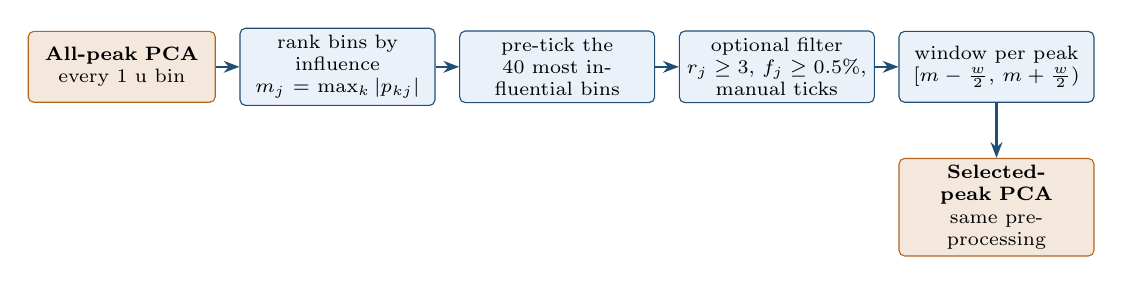
\begin{tikzpicture}[node distance=3mm]
    \node[hw,text width=2.2cm] (a) {\textbf{All-peak PCA}\\every 1~u bin};
    \node[box,text width=2.3cm,right=of a] (b) {rank bins by influence\\$m_j=\max_k|p_{kj}|$};
    \node[box,text width=2.3cm,right=of b] (c) {pre-tick the 40 most influential bins};
    \node[box,text width=2.3cm,right=of c] (d) {optional filter $r_j\ge3$, $f_j\ge0.5\%$, manual ticks};
    \node[box,text width=2.3cm,right=of d] (e) {window per peak $[m-\tfrac w2,\,m+\tfrac w2)$};
    \node[hw,text width=2.3cm,below=7mm of e] (f) {\textbf{Selected-peak PCA}\\same preprocessing};
    \foreach \x/\y in {a/b,b/c,c/d,d/e} \draw[arr] (\x) -- (\y);
    \draw[arr] (e) -- (f);
  \end{tikzpicture}
  \vspace{3mm}
  \begin{itemize}\setlength\itemsep{2mm}
    \item The user can add or remove peaks and subsamples by hand. The choice is passed live to the second tab.
    \item Both PCAs give scree, scores of every PC pair with 90\% ellipses per label group, and loadings.
  \end{itemize}
\end{frame}

\begin{frame}{Real data: scores, All-peak vs Selected-peak}
  \begin{columns}[T]
    \begin{column}{0.5\textwidth}
      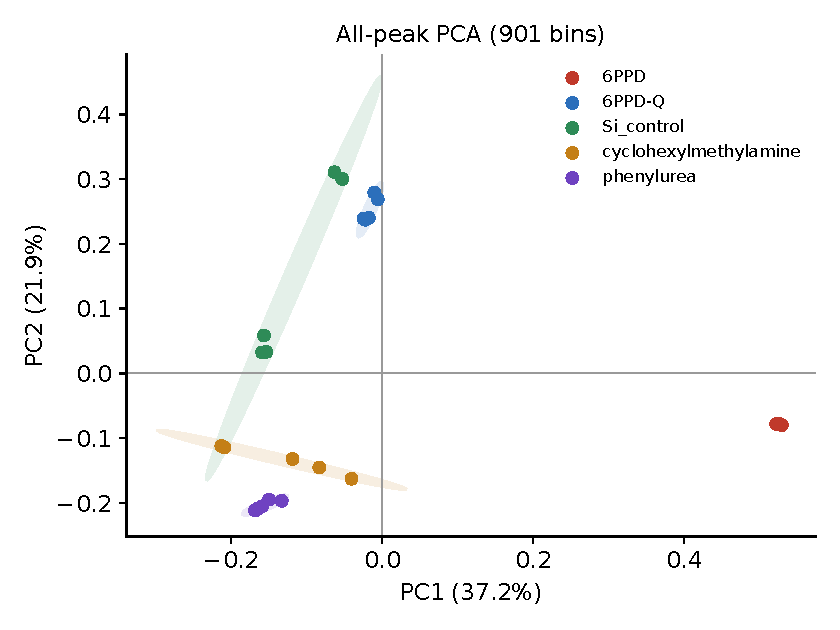
\includegraphics[width=\textwidth]{scores_all.pdf}
    \end{column}
    \begin{column}{0.5\textwidth}
      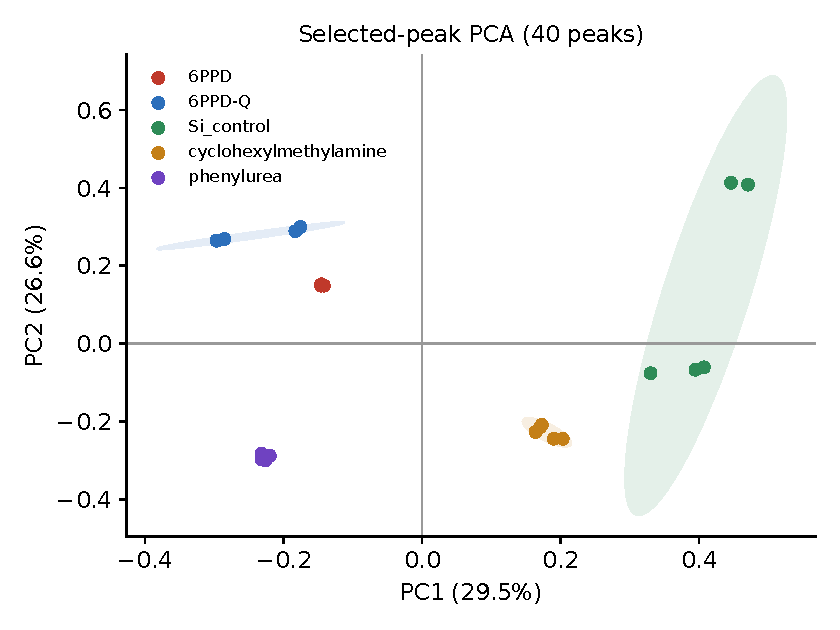
\includegraphics[width=\textwidth]{scores_sel.pdf}
    \end{column}
  \end{columns}
  \vspace{-1mm}
  {\scriptsize 24 subsamples, positive polarity, normalised, square root, mean-centred. Shaded ellipse: 90\% of each label group (groups with fewer than three points or on a line have none).}
  \begin{itemize}\setlength\itemsep{1mm}
    \item The five groups are distinguishable in both PCAs. In the All-peak PCA, 6PPD is far from the rest on PC1.
  \end{itemize}
\end{frame}

\begin{frame}{Real data: loadings of PC1}
  \begin{columns}[T]
    \begin{column}{0.5\textwidth}
      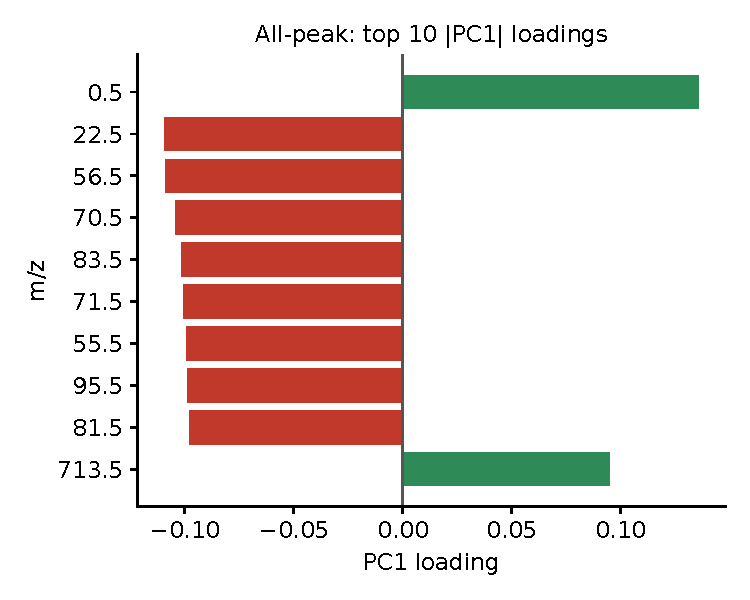
\includegraphics[width=\textwidth]{loadings_all.pdf}
    \end{column}
    \begin{column}{0.5\textwidth}
      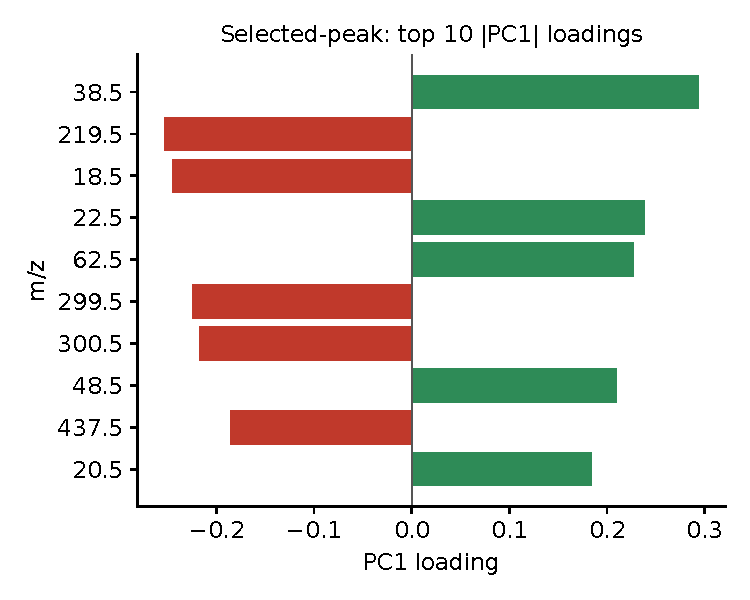
\includegraphics[width=\textwidth]{loadings_sel.pdf}
    \end{column}
  \end{columns}
  \vspace{-1mm}
  {\scriptsize m/z is the bin centre. Green: positive loading, red: negative.}
  \begin{itemize}\setlength\itemsep{1mm}
    \item Loadings tell which bins separate the samples on PC1. Their identity (which ion) is then checked against the peak table.
  \end{itemize}
\end{frame}

\begin{frame}{Real data: numbers}
  \begin{columns}[T]
    \begin{column}{0.5\textwidth}
      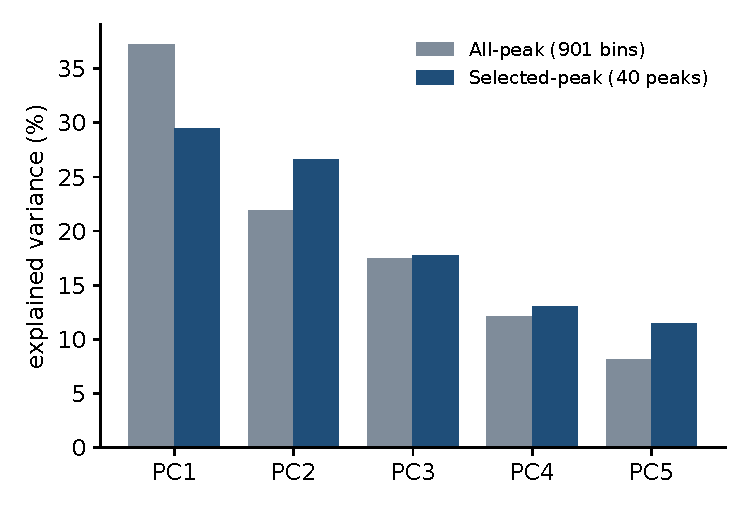
\includegraphics[width=\textwidth]{scree.pdf}
    \end{column}
    \begin{column}{0.5\textwidth}
      \small
      \begin{tabular}{@{}lrr@{}}
        \toprule & All-peak & Selected-peak\\\midrule
        features & 901 bins & 40 peaks\\
        PC1 & 37.2\% & 29.5\%\\
        PC2 & 21.9\% & 26.6\%\\
        PC1 + PC2 & 59.1\% & 56.1\%\\
        PC1 to PC5 & 96.8\% & 98.2\%\\\bottomrule
      \end{tabular}\\[3mm]
      \scriptsize The 40 selected bins hold 17.6\% of all ions.
    \end{column}
  \end{columns}
\end{frame}

\begin{frame}{How our tool differs from Yang et al.}
  \small
  \begin{tabular}{@{}>{\raggedright\arraybackslash}p{3.5cm}>{\raggedright\arraybackslash}p{4.1cm}>{\raggedright\arraybackslash}p{4.9cm}@{}}
    \toprule & \textbf{Yang et al.\ 2019} & \textbf{This tool}\\\midrule
    Mass calibration & done in the instrument software & done upstream, data already calibrated\\
    Interference (PDMS, Bi) & removed before ``all peak'' & \hl{not removed}: every bin is a feature\\
    Medium overlay ($>90\%$) & used to build ``selected peak'' & \hl{not implemented} (needs a medium or matrix sample)\\
    
  \end{tabular}
  \vspace{3mm}
  \begin{itemize}\setlength\itemsep{1.5mm}
    \item The selected peaks are picked from the same data they are then analysed on.
    
  \end{itemize}
\end{frame}

\begin{frame}{Take-home}
  \begin{itemize}\setlength\itemsep{3mm}
    \item \hl{PCA} turns a spectrum table into a few axes: \hl{scores} show which samples differ, \hl{loadings} show which peaks make the difference.
    \item Spectra are first transformed: \hl{total-ion normalisation $\rightarrow$ square root $\rightarrow$ mean centring}. No z-score, no logarithm.
    \item \hl{Two rounds} (Yang et al.): All-peak PCA first, then Selected-peak PCA on a reduced, curated peak list. \hl{Peak selection changes the interpretation}.
    \item Selection tests (Fu et al.): $\ge3\times$ neighbours and $>0.5\%$ of the ions, implemented as $r_j$ and $f_j$.
  \end{itemize}
\end{frame}

\begin{frame}{References}
  \footnotesize
  \begin{itemize}\setlength\itemsep{3mm}
    \item C.~Yang, W.~Wei, F.~Liu, X.-Y.~Yu. Peak selection matters in principal component analysis: A case study of syntrophic microbes. \emph{Biointerphases} 14, 051004 (2019). doi:10.1116/1.5118237
    \item Y.~Fu, Y.~Zhang, F.~Zhang, J.~Chen, Z.~Zhu, X.-Y.~Yu. Does interfacial photochemistry play a role in the photolysis of pyruvic acid in water? \emph{Atmospheric Environment} 191, 36--45 (2018). doi:10.1016/j.atmosenv.2018.07.061
    \item K.~L.~Sek, P.~L.~Lee, K.~Y.~Pang, Y.~Hua, L.~Zhu, X.~Li. Principal Component Analysis (PCA) of Surface Contamination by TOF-SIMS. \emph{IEEE IPFA} (2021). doi:10.1109/IPFA53173.2021.9617378
  \end{itemize}
\end{frame}

\end{document}
